% !TeX spellcheck = pl_PL
\newpage
\section{USB – Uniwersalny interfejs szeregowy}
	\subsection{Zalety}
	\begin{itemize}
		\item Podłączenie dużej liczby różnorodnych urządzeń
		\item Automatyczne wykrywanie włączenia urządzenia do systemu oraz jego odłączenia
		\item Przeprowadzanie wszystkich operacji konfiguracyjnych, w tym instalacji sterownika, bez udziału użytkownika
		\item Szybka transmisja
		\item Zasilanie urządzenia bezpośrednio z portu
	\end{itemize}
	\subsection{Parametry}
	Dla USB 1.1 oraz 2.0
	\begin{itemize}
		\item Szybkość transmisji: 12 Mb/s (1.1), 480 Mb/s (2.0)
		\item Złożoność kontrolera w stacji host: 10000 bramek
		\item Złożoność kontrolera w urządzeniu: 1500 do 2000 bramek
	\end{itemize}
	\subsection{Charakterystyka systemu USB}
		\subsubsection{Podstawowe właściwości interfejsu USB}
		\begin{itemize}
			\item \textbf{Gorące podłączenie} - włączanie/wyłączanie urządzeń bez wyłączania systemu oraz konfiguracja bez udziału użytkownika.
			\item \textbf{Jeden typ złącza} - złącze typu A w koncentratorze i B w urządzeniu (dwa kontakty linii danych oraz dwa zasilania).
			\item \textbf{Duża liczba podłączanych urządzeń} - moduły komunikacyjne, jak hub czy koncentrator, posiadają kilka portów USB oraz umożliwiają łączenie kaskadowe w celu rozszerzenia liczby portów do podłączanie urządzeń. W ten sposób można uzyskać wielopoziomową gwieździstą strukturę.\\Ostatecznie do USB można podłączyć maksymalnie \textbf{127} urządzeń.
			\item \textbf{Różne szybkości transmisji}
			\begin{itemize}
				\item Mała (\emph{low speed}): 1,5 Mb/s
				\item Pełna (\emph{full speed}): 12 Mb/s
				\item Wysoka (\emph{high speed}): 480 Mb/s
			\end{itemize}
			\item \textbf{Zasilanie} - USB posiada własny system dystrybucji zasilania: minimalnie dostarcza 4.7 V/100 mA (zagwarantowane przez magistralę), maksymalnie 500 mA (przy zasilaniu zewnętrznym lub hybrydowym). Przy braku aktywnosci na magistrali przez 3s urządzenia przechodzą w tryb zmniejszonego poboru prądu (SUSPEND), gdzie mogą pobierać maksymalnie 500 $\mu A$. Wyjście z tego trybu jest możliwe poprzez inicjatywę hosta bądź urządzenia (\emph{remote wake-up})
			\item \textbf{Protokół komunikacyjny, detekcja błędów} - obowiązuje złożony, pakietowy protokół k. z kontrolą poprawności przesyłu. Żądania przesłania danych (\emph{transfer}) dzielone są na transakcje , które z kolei złożone są z pakietów: kontrolnego, danych i potwierdzenia. Pakiety są zabezpieczone sumą kontrolną. W przypadku wykrycia błędu jest możliwe powtórzenie transakcji.
			\newpage
			\item \textbf{Transfery USB} - 4 typy transferów:
				\begin{itemize}
					\item Kontrolny (\emph{control transfer})
					\item Masowy (\emph{bulk transfer})
					\item Przerwaniowy (\emph{interrupt transfer})
					\item Izochroniczny (\emph{isochronous transfer})
				\end{itemize}
			\item \textbf{Niski koszt} - nieduża złożoność układów interfejsowych
			\item \textbf{Schemat blokowy systemu USB}\\
			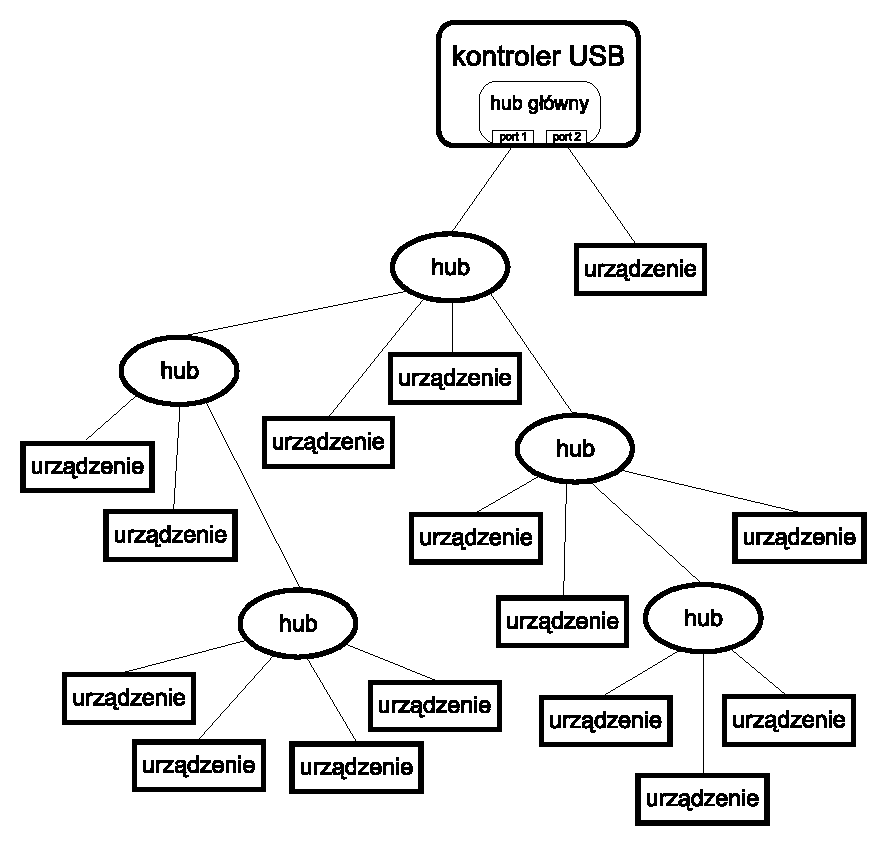
\includegraphics[width=12cm]{./wyklady/USB_6_1.pdf}
		\end{itemize}
		\subsubsection{Środowisko sygnałowe}
			Łącze transmisyjne oparte jest na obwodzie różnicowym. Różnicowy nadajnik jest połączony z różnicowym odbiornikiem przez parę przewodów.\\
			W przypadku transmisji wolnej wystarcza para nieskręcana i nieekranowana, natomiast transmisja pełna lub wysoka wymaga pary skręcanej i ekranowanej.\\
			Zasilanie jest przekazywane przewodami $V_{cc} (+5V)$ oraz $GND$ (masa).\\
			Trójstanowy nadajnik można zablokować sygnałem OE, co oznacza blokadę portu. Wówczas wyjście nieodwracające (D+) i odwracające (D-) przy zablokowanym nadajniku zostają na potencjale masy (patrz rezystory 15k).\\
			Wzmacniacze odniesione do masy monitorują napięcie na liniach D+ i D-.
		\newpage
			\textbf{Obwód transmisyjny w standardzie USB}\\
			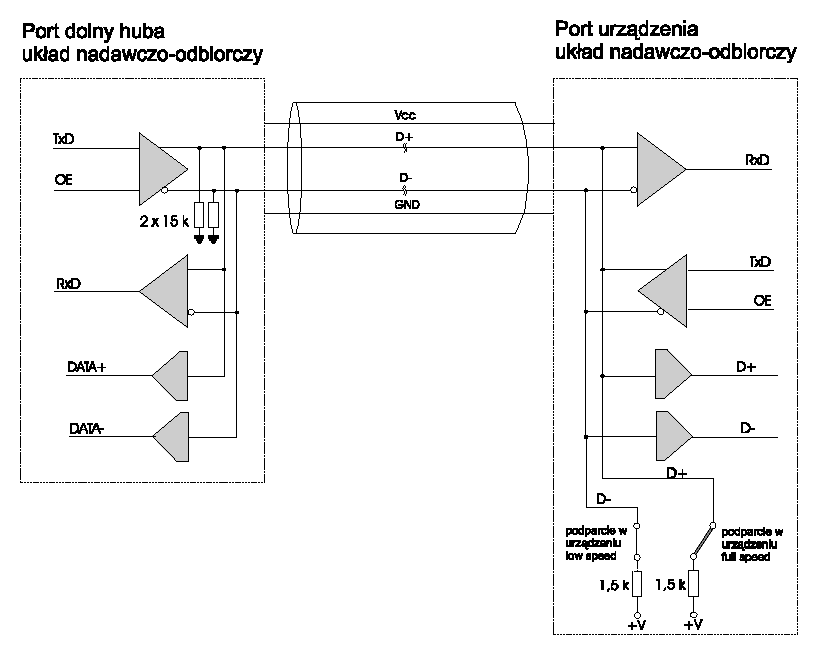
\includegraphics[width=9cm]{./wyklady/USB_7_1.pdf}\\
			\textbf{Stany magistrali USB}\\
			\begin{itemize}
				\item Logiczne „1” w obwodzie różnicowym (D+) - (D-) $>$ 200 mV
				\item Logiczne „0” w obwodzie różnicowym (D+) - (D-) $<$ -200 mV
				\item Plus 9 innych stanów
			\end{itemize}
			\textbf{Kodowanie bitów w systemie USB}\\
			W systemie USB przyjęto kodowanie NRZI (\emph{Non Return to Zero Inteverted}) ze wstawianiem bitu synchronizującego (tzw. \emph{bit stuffing}). Na początku każdego bitu o wartości logicznej zero następuje zmiana sygnału, natomiast po każdych 6 kolejnych bitach o wartości jeden wstawiany jest bit o wartości zero. Umożliwia to prawidłowe poznawanie bitów w sygnale odebranym bez potrzeby przesyłania sygnału zegarowego nadajnika. Bity wstawione są usuwane po rozpoznaniu stanu bitów w odebranym sygnale.\\\\
			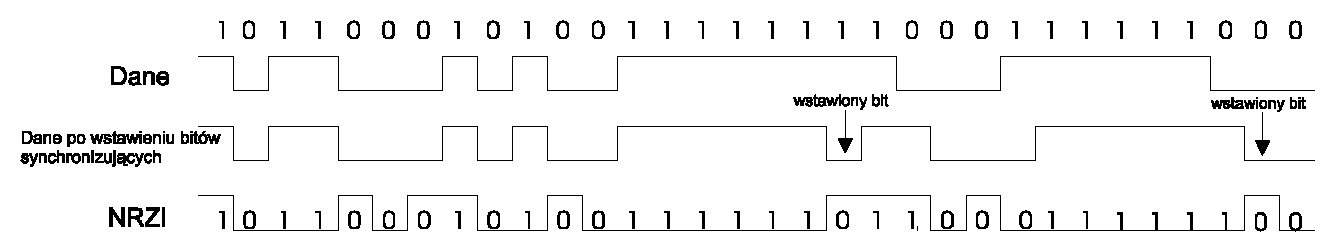
\includegraphics[width=15cm]{./wyklady/USB_9_1.pdf}
		\subsubsection{Środowisko fizyczne}
			\textbf{Podstawowy kabel do podłączenia urządzenia USB}\\
			\begin{wrapfigure}{l}{8cm}
				\vspace{-20pt}
				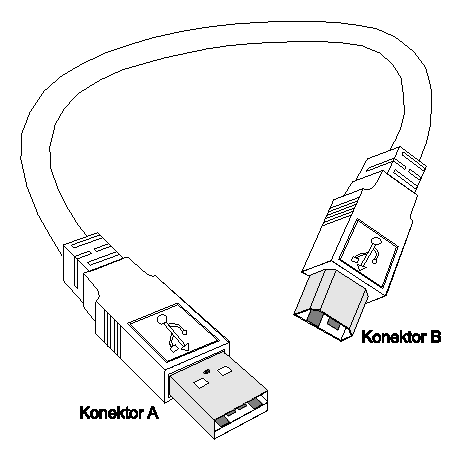
\includegraphics[width=6cm]{./wyklady/USB_10_1.pdf}
			\end{wrapfigure}
			W standardzie USB wyróżnia się dwa rodzaje złączy
			\begin{itemize}
				\item Konektor A – strona portu dolnego (hub), "od strony urządzenia"
				\item Konektor B – strona portu górnego (urządzenie), "od strony hosta"
			\end{itemize}
			Złącza USB posiadają 4 zaciski: po dwa dla magistrali danych i zasilania. W samym złączu kontakty zasilania są nieco wysunięte w przód przed kontakty danych, a więc po włożeniu najpierw jest podłączone zasilanie, a potem dane.
			\clearpage
			\begin{table}[H]	%H z pakietu 'float' wymusza polozenie HERE  (bez tego zle ulozenie trsci)
				\begin{tabular}{|c|c|c|}
					\hline
					\textbf{Nr kontaktu}	& \textbf{Nazwa sygnału}	& \textbf{Kolor przewodu w kablu} \\ \hline
					1 						& Vcc						& Czerwony		\\ \hline
					2 						& +DATA						& Biały			\\ \hline
					3 						& -DATA						& Zielony		\\ \hline
					4 						& GND						& Czarny		\\ \hline
				\end{tabular}
			\end{table}
		
		\subsubsection{Rodzaje kabli}
			\begin{itemize}
				\item Kabel przeznaczony dla urządzeń „low speed”
				\begin{itemize}
					\item Nieekranowany
					\item Zawiera dwie, nieskręcane pary przewodów: dla danych (28 AWG) i zasilania (20-28 AWG)
				\end{itemize}
				\item Kabel przeznaczony dla urządzeń „full speed i high speed”
				\begin{itemize}
					\item Zawiera ekranowaną parę skręcaną (28 AWG) dla danych
					\item I nieekranowaną parę (20-28 AWG) dla zasilania
				\end{itemize}
				\item Czas propagacji sygnału w kablu: $<$ 30 ns przy przesyle z częstotliwością 1-16 MHz. Wymagany dla urządzeń małej i pełnej szybkości. Czas propagacji wpływa na długosc kabla:
				\begin{itemize}
					\item 5 m dla 6ns/m
					\item 3 m dla 10ns/m
				\end{itemize}
			\end{itemize}
		\subsubsection{Ramki i mikro ramki}
			W systemie USB dane są przekazywane:
			\begin{itemize}
				\item W ramkach o czasie trwania 1 $ms$ dla małej i pełnej szybkości transmisji.
				\item W mikroramkach o czasie trwania 125 $\mu s$ dla wysokiej szybkości transmisji.
			\end{itemize}
			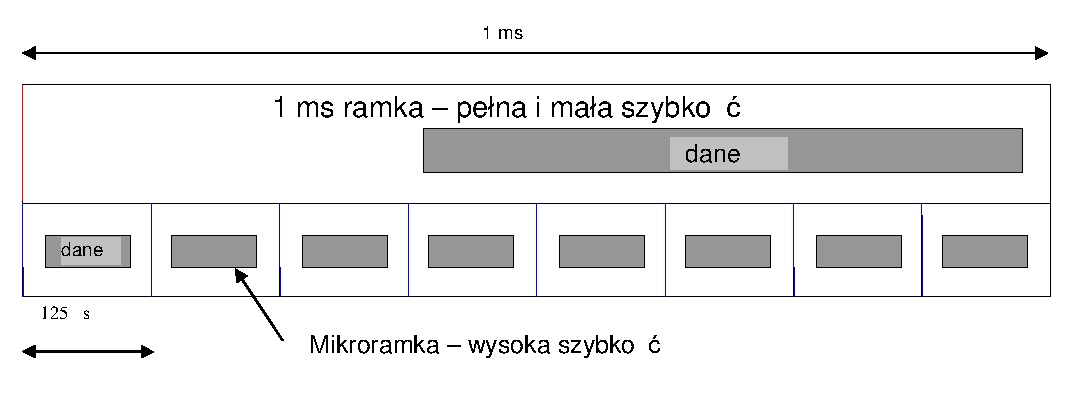
\includegraphics[width=10cm]{./wyklady/USB_11_1.jpg}\\
			\textbf{Ramka 1 ms}
			\begin{itemize}
				\item Czas pomiędzy dwoma kolejnymi pakietami SOF (\emph{Start Of Frame}) nazywany jest ramką. Początek ramki wyznacza pakiet SOF zawierający 11 bitów danych i 5 bitów CRC. Dane w pakiecie SOF reprezentują kolejny numer ramki. Licznik ramek przepełnia się co 2048 ms.
				\item Pełna szybkość transmisji
				\begin{itemize}
					\item Maksymalny teoretyczny rozmiar ramki w bitach: 1 ms x 1/12 Mhz = 12000 bitów
					\item Powyższy rozmiar ramki w bajtach: 12000 : 8 = 1500.
					\item Pakiety kontrolne zajmują ok. 300 bajtów.
					\item Praktyczna górna granica liczby transmitowanych w ramce: 1200 bajtów.
				\end{itemize}
				\item Mała szybkość transmisji
				\begin{itemize}
					\item Max rozmiar ramki w bitach: 1 ms x 1/1,5 Mhz = 1500 bitów
					\item Max rozmiar ramki w bajtach: 1500 : 8 = 187
				\end{itemize}
			\end{itemize}
			\newpage
			\textbf{Mikroramka 125 $\mu s$}
			\begin{itemize}
				\item Czas pomiędzy dwoma kolejnymi pakietami SOF wysyłanymi przez high speed huba nazywa się mikroramką.
				\item Mikroramka trwa 125 $\mu s$
				\item Na 1 ramkę przypada 8 mikroramek
				\item Wysoka prędkość transmisji - szybkość transmisji w mikroramce wynosi 480 Mhz.
			\end{itemize}
			
		\subsubsection{Model komunikacyjny}
		Warstwowy model komunikacyjny przedstawiający odpowiadające sobie elementy sprzętowo-programowe po stronie hosta i urządzenia.\\
		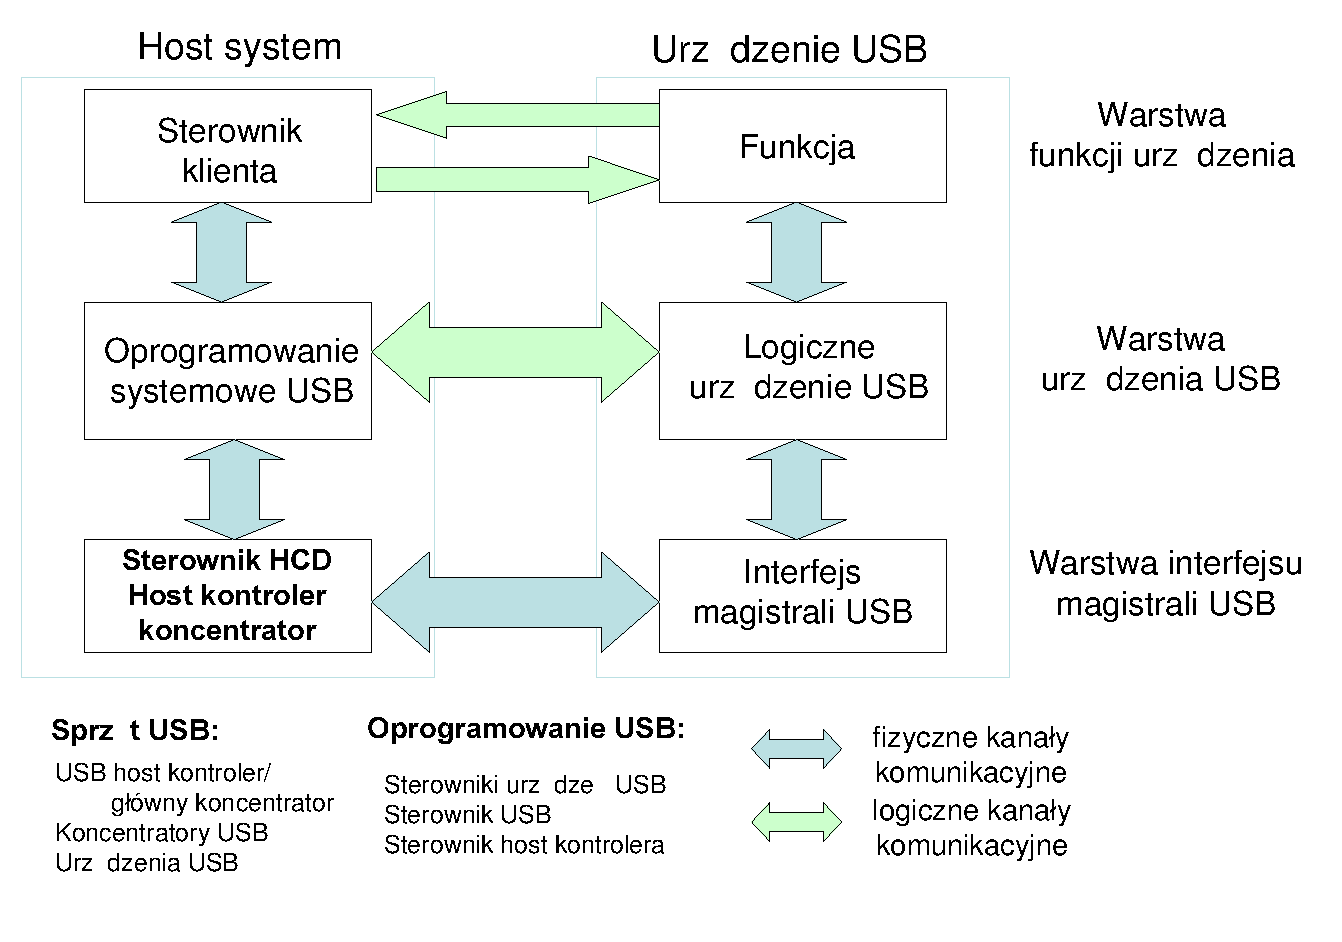
\includegraphics[width=10cm]{./wyklady/USB_12_1.jpg}\\\\
		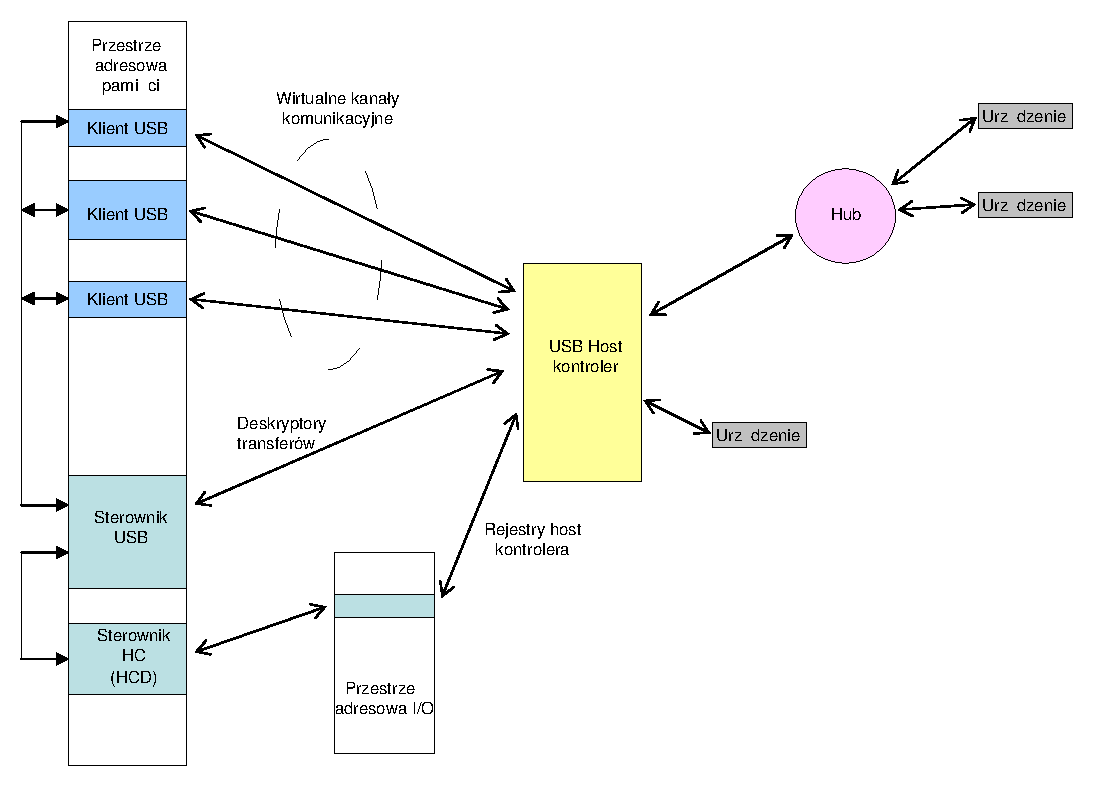
\includegraphics[width=10cm]{./wyklady/USB_13_1.jpg}\\
		\newpage
		\subsubsection{Transfery USB}
		Wyróżniono 4 typy transferów przeznaczone dla rożnych urządzeń z różnymi wymaganiami komunikacyjnymi. Każdy wymaga innego kanału komunikacyjnego (\emph{pipe}).
		\begin{itemize}
			\item \textbf{Masowy} (\emph{bulk transfer}) - time delivery accuracy + quality delivery accuracy ("jak najlepiej w miarę możliwości").\\
			Przeznaczony do komunikacji z urządzeniami, do których zapisuje się lub z których odczytuje duże ilości danych, jednak czas przekazywania danych oraz regularność ich dostarczania nie są krytyczne.\\
			Ważna jest kontrola przekazywanych danych, błędy transmisji muszą zostać wykryte i skorygowane poprzez żadanie ponownego przesłania błędnego bloku danych.\\
			Nie ma zagwarantowanego pasma, transmisja ta jest realizowana, jeżeli inne transfery nie wykorzystają przydzielonych im zasobów.\\
			Może być realizowany tylko z pełną lub wysoką szybkością.\\
			Wymagane jest, aby pakiet danych miał stałą wartość (\emph{MaxPacketSize}): 8, 16, 32 lub 64. Wszystkie kolejne pakiety danych muszą mieć tę stałą wartość z wyjątkiem ostatniego, który sygnalizuje koniec transferu.
			Przykłady: drukarka, skaner.
			\item \textbf{Przerwaniowy} (\emph{interrupt transfer}) - quality delivery accuracy.\\
			Do komunikacji z urządzeniami, do których zapisuje się lub z których odczytuje się niewielkie bloki danych, jednak trzeba robić to regularnie, w ustalonych odstępach czasowych.\\
			Parametry transferu zawarte są w deskryptorze pobieranym na etapie konfiguracji urządzenia.\\
			Ma zagwarantowane pasmo, może być wykorzystany do obsługi urządzeń low speed i full speed.\\
			Rozmiar pakietu danych zależy od wybranej szybkości: dla low speed jest to 8, dla full speed to maksymalnie 64. Wszystkie kolejne pakiety danych muszą mieć tę stałą wartość z wyjątkiem ostatniego, który sygnalizuje koniec transferu.\\
			Przykłady: mysz, klawiatura.
			\item \textbf{Izochroniczny} (\emph{isochronous transfer}) - time delivery accuracy.\\
			Przeznaczony do komunikacji z urządzeniami, do których zapisuje się lub z których odczytuje duże ilości danych, przy czym krytyczna jest regularność dostarczania danych.\\
			Nie jest ważna kontrola przekazywania danych, nie jest dopuszczalne ponowne wysłanie bloku danych.\\
			Dla komunikacji w pełnej lub wysokiej szybkości. Parametry transferu USB odczytuje z deskryptora urządzenia.\\
			Graniczna wartość parametru \emph{MaxPacketSize} to 1023 bajty na ramkę.\\
			Przykład: odtwarzanie muzyki w aparaturze audio.
			\item \textbf{Kontrolny} (\emph{control transfer}) - time delivery accuracy + quality delivery accuracy.\\
			Musi być obsługiwany przez każde urządzenie USB, ponieważ jest przeznaczony do jego konfiguracji i nadzoru. W ramce zarezerwowano stosowane pasmo dla realizacji transferów kontrolnych (10\% czasu trwania ramki).\\
			Obsługuje wszystkie 3 rodzaje prędkości transferu.\\
			Dzieli się na 3 etapy:
			\begin{itemize}
				\item Przekazanie rozkazu - 8-bitowe pole danych udostępnia informację o liczbie bajtów danych przesyłanych w etapie przekazani danych, o ile ten występuje.
				\item Przekazanie danych - pakiety danych mogą mieć rozmiar nie większy niż 64 bajty (parametr \emph{MaxPacketSize}).
				\item Przekazanie statusu.
			\end{itemize}
		\end{itemize}
		\newpage
		\textbf{Podział i podsumowanie transferów}
		\begin{table}[h]
			\begin{tabular}{|p{4cm}|p{3cm}|p{3cm}|p{3cm}|p{3cm}|}
				\hline
				\textbf{Cechy i parametry} & \textbf{Kontrolny}	   & \textbf{Masowy} & \textbf{Przerwaniowy} & \textbf{Izochroniczny} \\ \hline
				Low speed (bajt/ms)  & 24 (3 transkacje 8 B)        & Nie dozwolony      			& 0,8 (8 B na 10 ms)		& nie dozwolony						\\ \hline
				Full speed (bajt/ms) & 832 (13 tr. 64 B na ramkę)   & 1216 (19 tr. 64 B na ramkę)   & 64 (1 tr 64 B na ramkę)	& 1023 (1 tr. 1023 B na ramkę)		\\ \hline
				High speed (bajt/ms) & 15872 (31 tr. 64 B na mikroramkę) & 53248 (13 tr. 512 B na mikroramkę) & 24576 (3 tr. 64 na mikroramkę)	& 24576 (3 tr. 64 B na mikroramkę)	\\ \hline
				Kierunek przepływu danych & Odczyt/zapis            & Odczyt/zapis       			& Odczyt/zapis		& Odczyt/zapis					\\ \hline
				Zarezerwowane pasmo  dla transferów w ramach ramki & 10\% dla low i full, 20\% dla high   & Brak rezerwacji  & 90\% dla low i full, 80\% dla high	& 90\% dla low i full, 80\% dla high	\\ \hline
				Kontrola błędów transmisji & Tak                	& Tak & Tak	& Nie	\\ \hline
				Komunikat/Strumień  & Komunikat		               & Strumień & Strumień   & Strumień	\\ \hline
				Określony rytm (periodyczność) & Aperiodyczny        & Aperiodyczny    & Periodyczny   & Periodyczny	\\ \hline
				\end{tabular}
		\end{table}
				\begin{itemize}
					\item Transfery strumieniowe (\emph{stream transfer}), przekazywanie danych bajt po bajcie.
					\item Transfery komunikatowe (\emph{message transfer}), struktura komunikatów i ich znaczenie określa standard.
				\end{itemize}
				
		\subsubsection{Zarządzenie magistralą USB}
		Wszystkie transfery USB są inicjowane i kontrolowane przez hosta. Host usiłuje jednocześnie realizować transfery wielu urządzeń tak, aby jedno urządzenie nie blokowało dostępu.\\ 
		Niektóre transfery mają priorytety. Transferom izochronicznym i przerwaniowym nadano 90\% pasma, a kontrolnym 10\%. Oznacza to, że transfer masowy nie jest gwarantowany - jeżeli pozostałe 3 rodzaje zajmą maksymalny możliwy czas, to transfer masowy się nie odbędzie.\\
		W praktyce jednak zdarza się to rzadko i 3 transfery nie wykorzystują pełnego pasma, co pozwala kontrolerowi USB na przydzielenie niewykorzystanego miejsca transferom masowym.\\
		Kontroler dąży do jak najlepszego wykorzystania miejsca w ramce, w które może wstawić nawet wiele transakcji danego transferu masowego.\\
		Działanie kontrolera oparte jest na zasadzie "usilnych starań" (\emph{best efforts}), aby jak najsprawniej (w jak najkrótszym czasie) zrealizować wszystkie żądane transfery. Jednak jeżeli w ramce 1 ms brakuje miejsca na transferu masowego to musi on czekać.
		\newpage
		\subsubsection{Stany urządzenia USB}
		Zanim urządzenie USB zostanie skonfigurowane i udostępnione aplikacjom musi przejść przez kilka stanów przestawionych na rysunku\\
		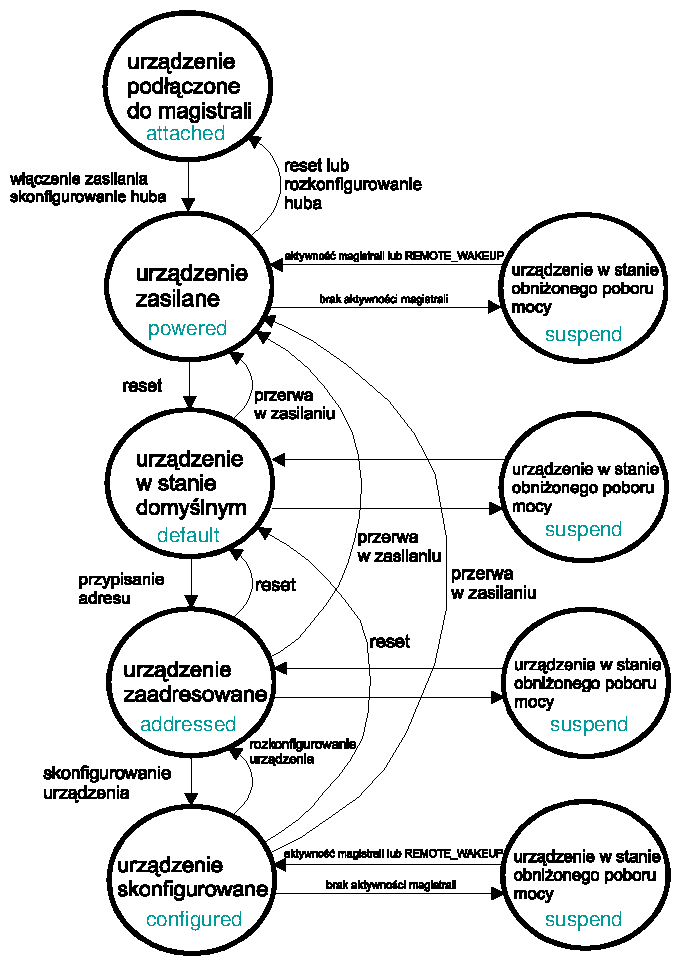
\includegraphics[width=10cm]{./wyklady/USB_16_1.pdf}
		\subsubsection{Hub w systemie USB}
		Huby to urządzenia pośredniczące w komunikacji z urządzeniami końcowymi.
		\begin{itemize}
			\item Zwiększają liczbę portów dostępnych dla urządzeń oraz możliwe jest ich kaskadowe łączenie.
			\item Port huba od strony hosta nazywa się górnym (\emph{uper stream port}), natomiast porty od strony urządzeń dolnym (\emph{down stream port}).
			\item Hub przeważnie posiada 4 porty dolne, rzadko kiedy inną liczbę jak np. 7.
			\item Hub nie tylko przekazuje dane, ale pośredniczy również w dystrybucji zasilania do urządzeń.
			\item Huby zgodne ze standardem 1.x są zdolne do komunikacji z małą lub pełną szybkością. Obowiązuje zasada, że do urządzeń low speed nie wolno kierować ruchu full speed. Hub potrafi wykryć jakie urządzenie jest podłączone do danego portu dolnego i wie, kiedy należy go zablokować.
			\item Transfery low speed są poprzedzone specjalną preambułą, których zadaniem jest odblokowanie portów dolnych do których podłączone są urządzenia low speed.
		\end{itemize}
		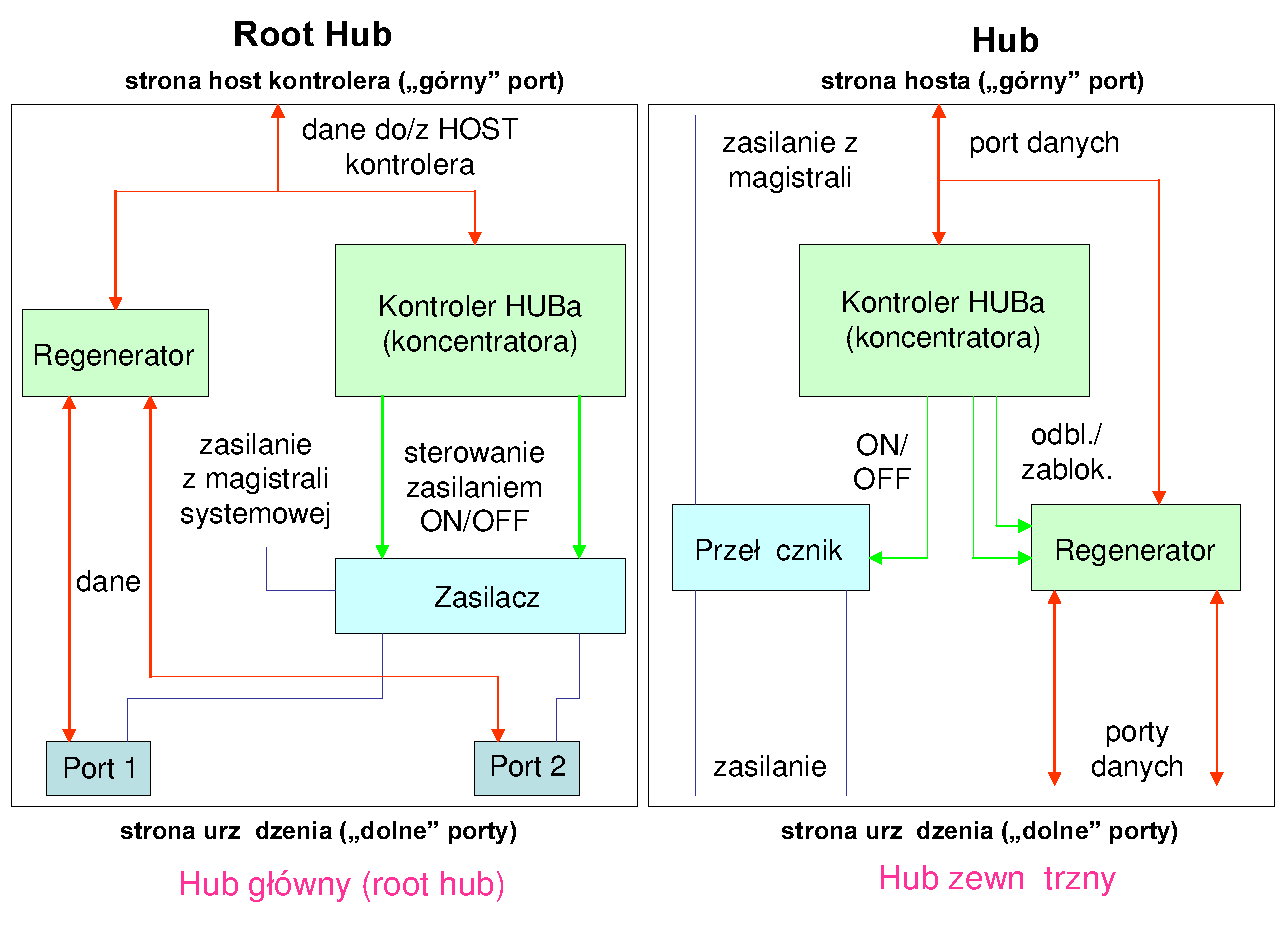
\includegraphics[width=10cm]{./wyklady/USB_17_1.jpg}
	
\subsection{Protokół komunikacyjny}
	Transakcje USB zbudowane sa z pakietów, przy czym typowa transakcja zawiera:
	\begin{itemize}
		\item Pakiet tokena (\emph{token packet}) - jest elementem kontrolnym transakcji i informuje o jej rodzaju: kontrolna lub przeznaczona do zapisywania danych.
		\item Pakiet danych (\emph{data packet}) - pole przeznaczone dla danych zapisywanych do urządzenia lub odczytywanych z urządzenia.
		\item Pakiet potwierdzenia (\emph{handshake packet}) - informuje jednostkę nadającą o odebraniu danych lub instrukcji sterującej przez odbiorcę.
	\end{itemize}
	\subsubsection{Właściwości}
	\begin{itemize}
		\item Komunikacja z urządzeniami USB za pomocą ramek o długości maksymalnie 1 ms.\\
		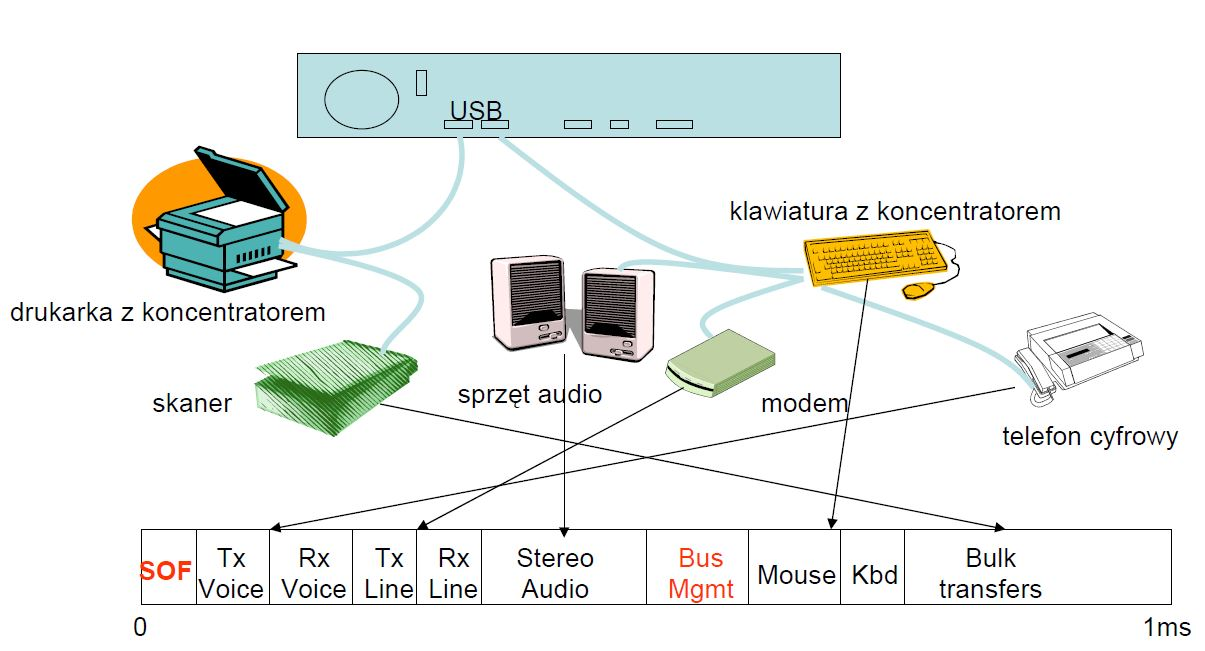
\includegraphics[width=10cm]{./wyklady/USB_18_1.jpg}
		\newpage
		\item Pakietowa struktura komunikatów\\
		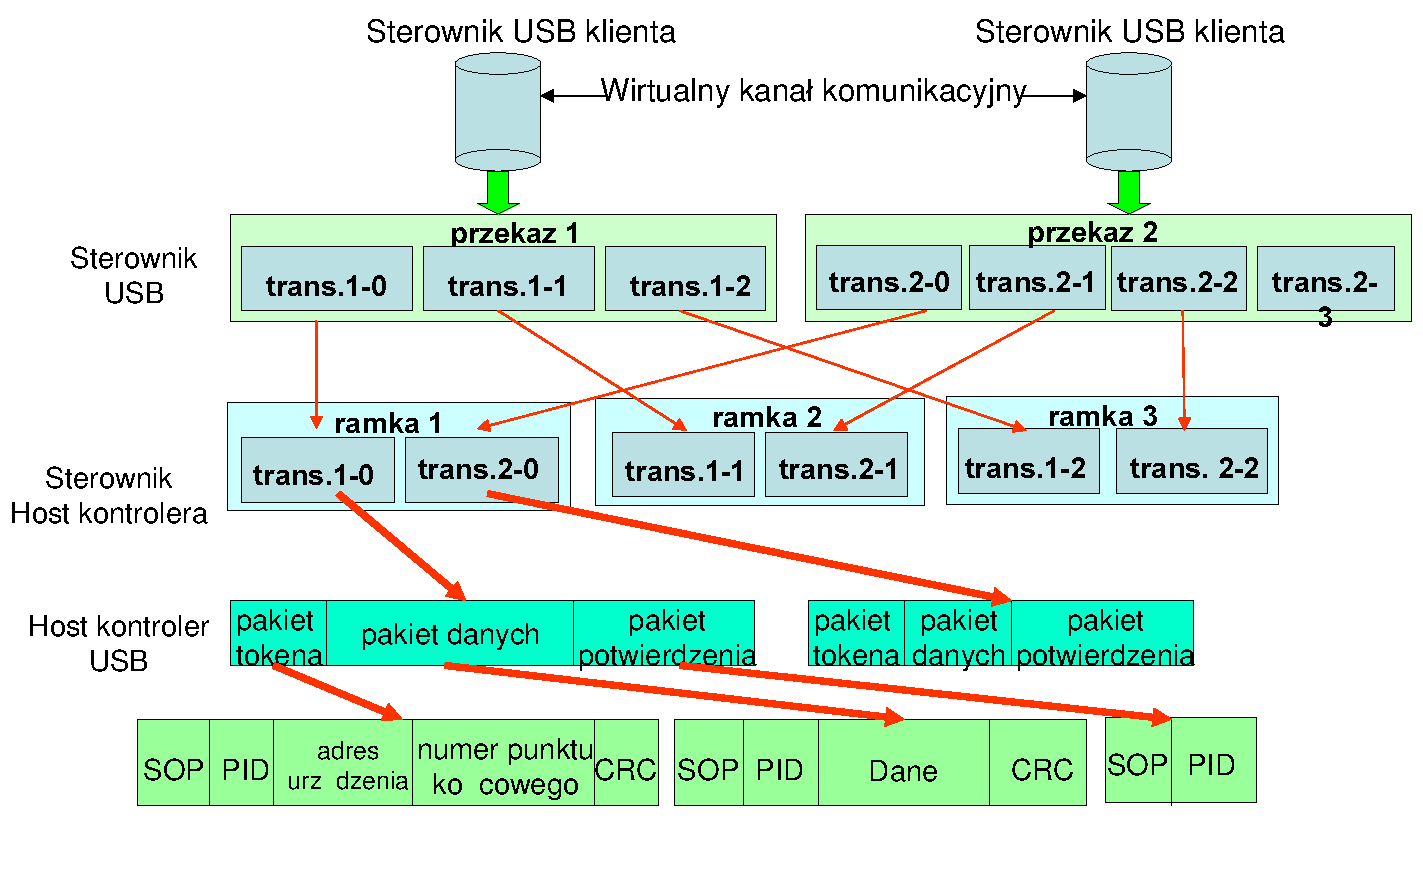
\includegraphics[width=10cm]{./wyklady/USB_19_1.jpg}\\
		Struktura bloków komunikacyjnych w USB (kolejkowanie odbywa się na poziomie sterownika host kontrolera)
	\end{itemize}
	\subsubsection{Format i typy pakietów USB}
	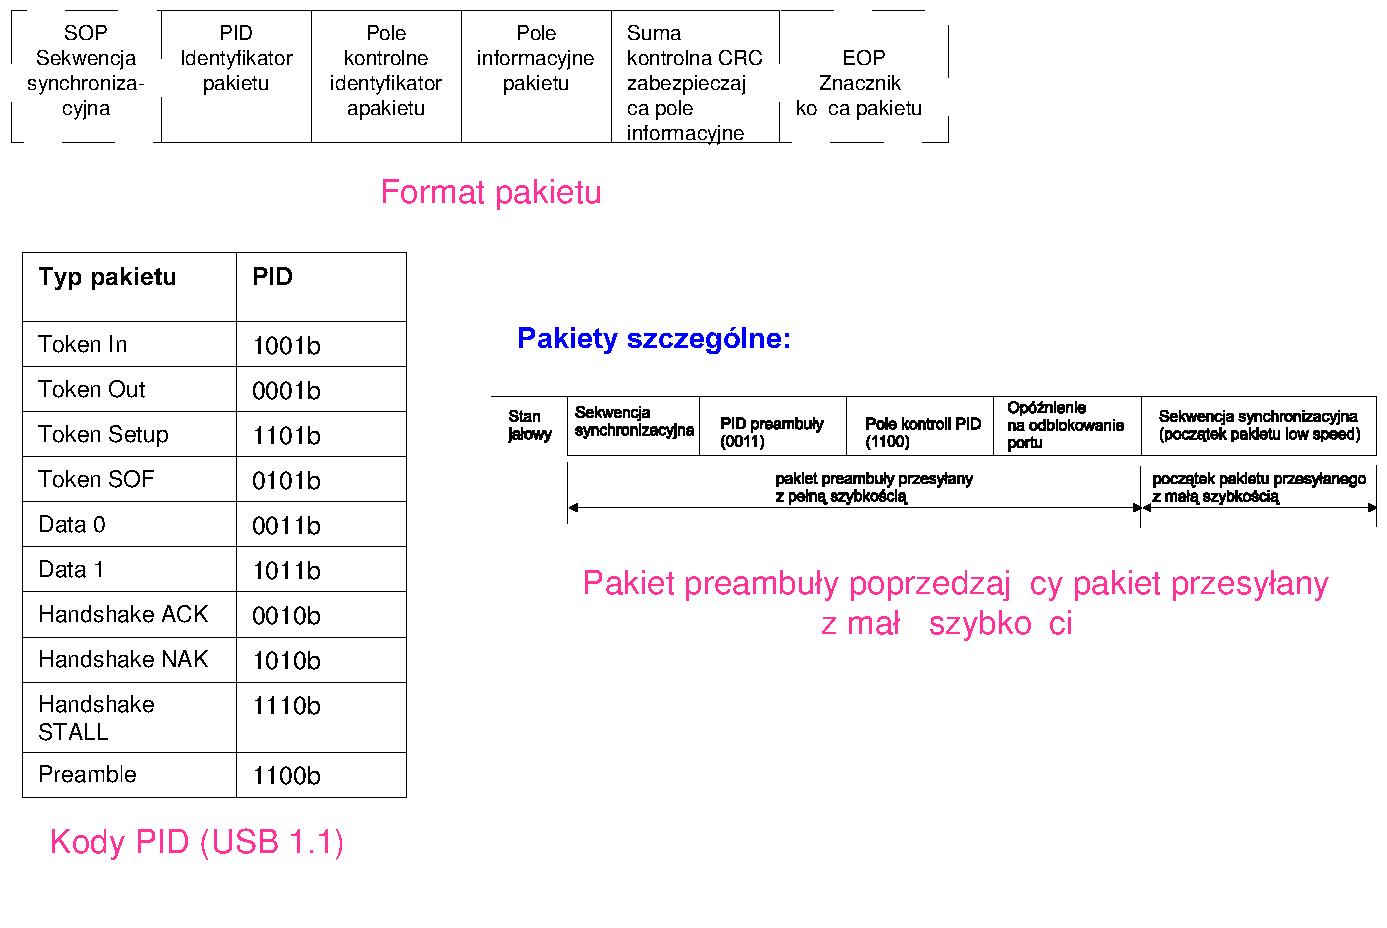
\includegraphics[width=10cm]{./wyklady/USB_20_1.jpg}
	\subsubsection{Reakcja na błędy}
	Wykrywanie błędów i kontrola transmisji\\
	\begin{itemize}
		\item Kontrola poprawności pakietów (zabezpieczenie pola PID sumą CRC)
		\begin{itemize}
			\item W przypadku pakietu Token - 5-bitowa suma
			\item W przypadku pakietu Data - 16-bitowa suma
		\end{itemize}
		Wykrycie błędu powoduje odrzucenie pakietu.
		\item Reakcja na fałszywy znacznik końca pakietu (\emph{false EOP})
		\item Ograniczenie czasowe oczekiwania na odpowiedź
		\item Przełączanie kolejnych pakietów danych (mechanizm \emph{data toogle})
		\item Wykrywanie transakcji występujących po zakończeniu ramki (tzw. „paplanie” – \emph{babble})
		\item Wykrywanie braku aktywności magistrali (LOA – \emph{Loss Of Activity})
	\end{itemize}
	Transfer kontrolny, przerwaniowy i masowy wysyłają pakiet ponownie, jeżeli jest on błędu, nie informując odbiorcy o tym. Transfer izochroniczny nie.
	\subsubsection{Czas obiegu (\emph{round trip delay})}
	Ograniczenie czasowe oczekiwania na odpowiedź. Jest to podstawowy mechanizm informowania nadawcy o niepoprawnym przekazaniu pakietu. Ograniczenie czasowe nie może być mniejsze od 16*(\emph{czas trwania bitu}), ani większe od 18*(\emph{czas trwania bitu}).\\
	Poniżej połączenie urządzenia z hostem przez 5 hubów – najgorszy przypadek pod względem czasowym.\\
	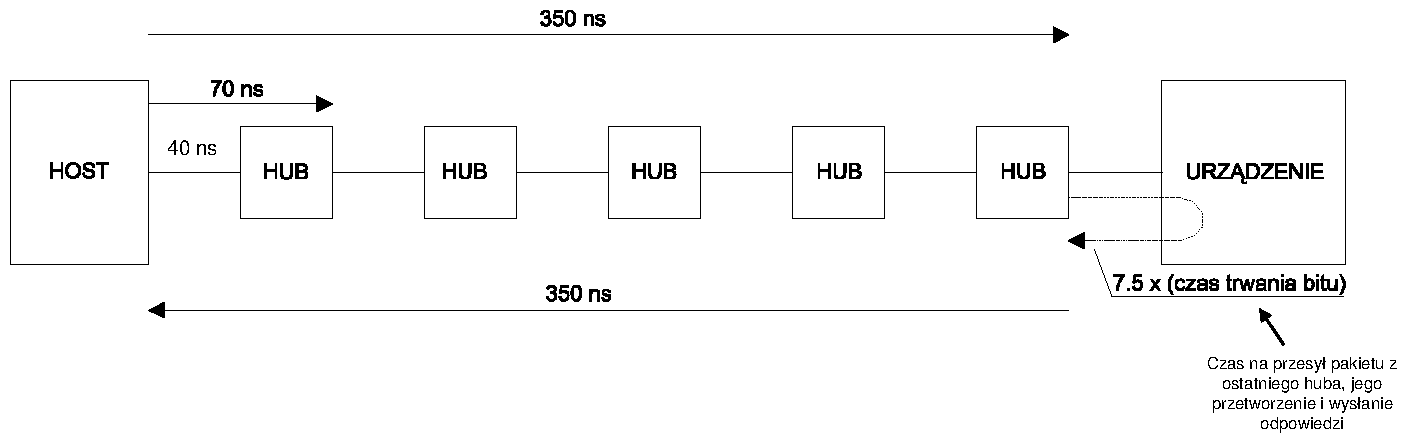
\includegraphics[width=10cm]{./wyklady/USB_23_1.pdf}\\
	Jest on podstawa do rozważań na temat ograniczeń tego czasu.
	\begin{itemize}
		\item Round trip delay: 2 x 350 ns = 700 ns
		\item Czas trwania 1 bitu dla full speed: 1/12 MHz = 83 ns
		\item Round trip delay w bitach dla full speed: 700 ns/83 ns = 8,5 bitu
		\item Timeout oczekiwania na odpowiedź: 7,5 bitu (specyfikacja) + 8,5 bitu = 16 bitów
	\end{itemize}
	
\subsection{Deskryptory w urządzeniach USB}
	W każdym urządzeniu USB znajduje się pełna informacja o sposobie komunikacji z urządzaniem, udostępniana podczas procesu enumeracji.\\
	Informacja ta jest przechowywana w deskryptorach - tablicach o ściśle określonej strukturze.
	\subsubsection{Hierarchiczna struktura deskryptorów w urządzeniu USB}
	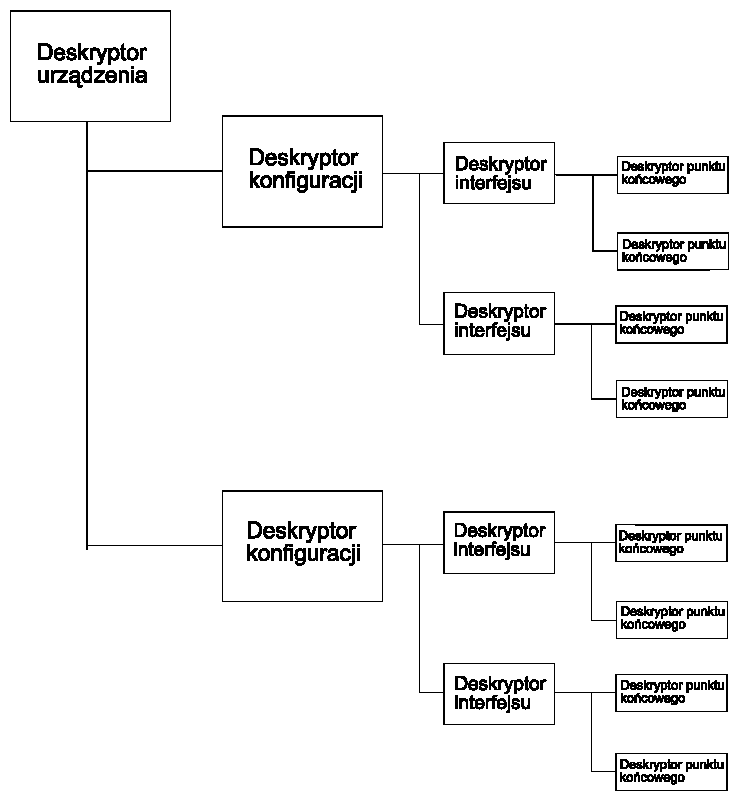
\includegraphics[width=10cm]{./wyklady/USB_24_1.pdf}
	\subsubsection{Rodzaje deskryptorów}
	\begin{itemize}
		\item Deskryptor urządzenia - m.in. liczba konfiguracji dostępnych w urządzeniu. (+ wersja USB, klasa, protokół, ID, wytwórca, nazwa produktu, nr seryjny)
		\item Deskryptor konfiguracji - opisuje każdą konfigurację z osobna. Zawiera informację o liczbie interfejsów przypisanych do danej konfiguracji oraz atrybuty zasilania, \textbf{maksymalny pobór prądu z krokiem co 2 mA}.
		\item Deskryptor interfejsu - posiada go każdy interfejs, który określa m.in. liczbę punktów końcowych z nim związanych.
		\item Deskryptor punktu końcowego - charakteryzuje każdy punkt końcowy. + adres, rodzaj transferu (\emph{bulk} itp.), odstęp czasowy odpytywania dla izochronicznego (1) i przerwaniowego (1-255)
		\item Deskryptor łańcuchowy - zawiera kod określający język tekstu lub sam właściwy tekst.
	\end{itemize}
	
	W danym urządzeniu może wystąpować maksymalnie jeden deskryptor urządzenia, oraz wiele deksryptorów innych rodzajów. Każdy deskryptor może posiadać parę pomniejszych deskryptorów.
	
\subsection{Wykrywanie i konfiguracja urządzeń}
	Cechą USB jest automatyczne wykrywanie urządzeń po włączeniu zasilania w systemie lub podłączeniu urządzenia do systemu. Procedura enumeracji zajmuje się rozpoznaniem urządzenia, sprawdzeniem czy komunikacja jest możliwa, przydzieleniem adresu, konfiguracją i instalacją sterownika.
	\subsubsection{Procedura enumeracji urządzenia}
	\begin{enumerate}
		\item Automatyczne wykrycie urządzenia - powoduje ustawienie bitu w rejestrze statusu huba, który odpowiada temu portowi.
		\item Odblokowanie portu i generacja RESETU - przejście do stanu domyślnego.
		\item Odczyt deskryptora urządzenia - skierowanie stosownego rozkazu do punktu końcowego 0 o adresie 0. Jest tylko jedno takie urządzenie w systemie - te, które właśnie podlega procesowi enumeracji.
		\item Przypisanie adresu - unikalny adres dla urządzenia
		\item Odczyt pozostałych deskryptorów - jeżeli istnieją
		\item Konfiguracja urządzenia
		\item Instalacja sterownika klienta
		\item Urządzenie jest dostępne dla aplikacji
	\end{enumerate}
	
\subsection{Kontrola urządzenia – transfer kontrolny}
	Transfer kontrolny służy do sterowania urządzeniem. Urządzenie USB otwiera kontrolny kanał komunikacyjny pomiędzy hostem a punktem końcowym 0 w urządzeniu.
	\subsubsection{Etapy transferu kontrolnego}
	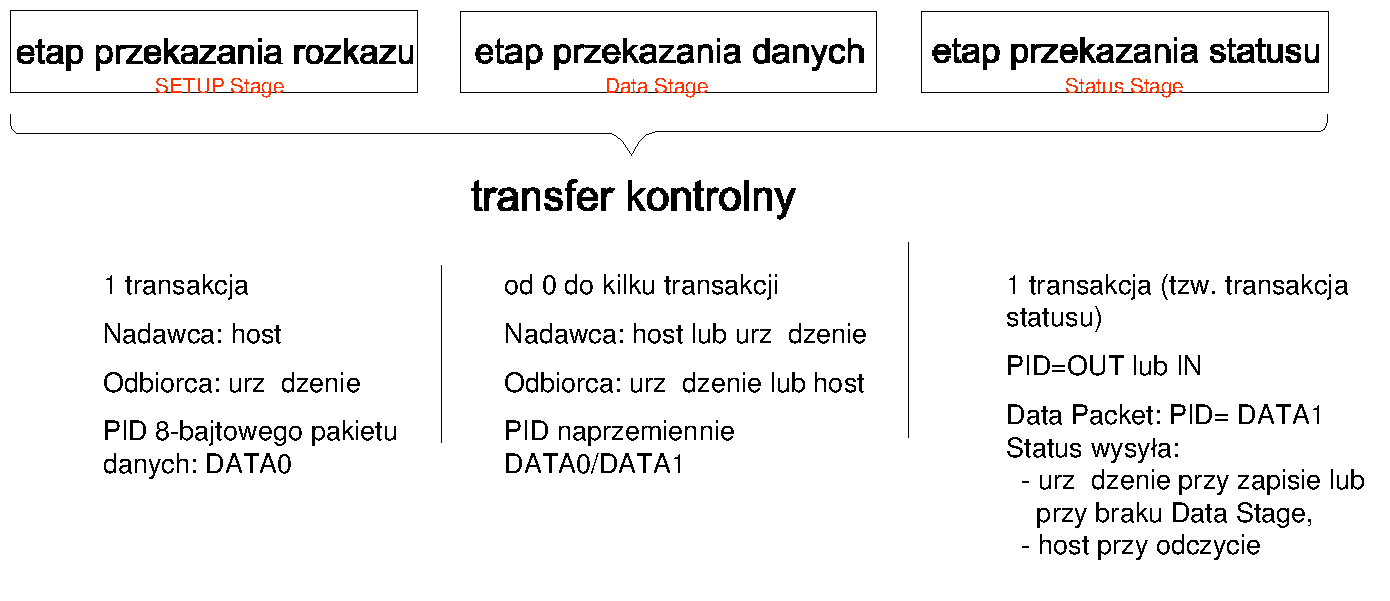
\includegraphics[width=10cm]{./wyklady/USB_31_1.pdf}
	\begin{enumerate}
		\item Przekazanie rozkazu (\emph{Setup Stage}) - jak w każdym pakiecie Token, następne pola zawierają adres urządzenia oraz punktu końcowego. Kolejnym elementem jest 8-bajtowy pakiet danych typu Data 0, który specyfikuje rozkaz. Transakcję kończy pakiet \emph{handshake}.
		\item Przekazanie danych (\emph{Data Stage}) - jeżeli 8 bajtów z powyższego nie wystarcza, wtedy następuje etap przekazania danych. Liczbę bajtów do przesłania określa słowo \emph{Length} w polu transakcji Setup. Jeżeli ta liczba nie przekracza wartości \emph{MaxPacketSize} to do przekazania danych wystarcza jedno transakcja, w przeciwnym razie odpowiednio dzieli się na więcej transakcji (sufit(Length / MPC)).\\
		Kodowanie:
		\begin{enumerate}
			\item Token packet IN (odczyt z urządzenia) / OUT (zapis).
			\item Data packet DATA0 (jeśli są następne, to naprzemiennie DATA1/DATA0)
			\item Handshake
		\end{enumerate}
		\item Przekazanie statusu (\emph{Status Stage}) - potwierdzenie wykonania transferu lub poinformowanie o niepowodzeniu w realizacji. Normalnie występuje do zakończeniu transakcji, ale host może rozpocząć ją wcześniej, w Data Stage (wtedy DS jest przerywane).
	\end{enumerate}
	
\subsection{Hub USB}
	\subsubsection{Co to jest?}
	Standard USB definiuje oddzielną klasę urządzeń: klasa HUB. Jest to tak ważna część tego systemu, że została zdefiniowana w standardzie USB, a nie we własnej oddzielnej specyfikacji.\\
	Typowy hub posiada jeden deskryptor.
	\subsubsection{HUB zasilany z magistrali}
	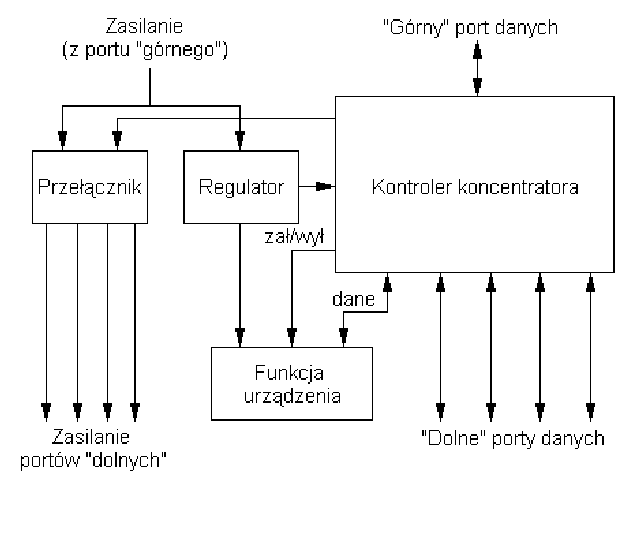
\includegraphics[width=10cm]{./wyklady/USB_34_1.pdf}
	\subsubsection{Proces konfiguracyjny huba}
	\begin{itemize}
		\item Odczyt standardowych deskryptorów urządzenia
		\item Przypisanie hubowi adresu
		\item Załączenie zasilania na porty, co jest niezbędne do detekcji podłączonych do portu urządzeń
		\item Odczyt punktu końcowego, "zmiany w hubie", w celu wykrycia urządzeń podłączonych do portów
		\item Odblokowanie portu w celu umożliwienia dostępu do urządzenia
	\end{itemize}
	\subsubsection{Punkt końcowy huba "zmiany w hubie"}
	\begin{itemize}
		\item Cyklicznie odczytywany, umożliwia monitorowanie zmian na portach dolnych huba, co z kolei umożliwia wykrywanie dołączania i usuwania urządzeń.
		\item Odpytywanie odbywa się przez wykorzystanie kanału przerwaniowego.
		\item \emph{Hub change point}: informuje o wystąpieniu:
		\begin{itemize}
			\item Zmiany w zasilaniu lub nadmiernym obciążeniu prądowym huba
			\item Zmiany na jednym lub kilku portach dolnych spowodowanej dołączeniem lub odłączeniem urządzenia.
		\end{itemize}
		\item Odczyt \emph{Hub change point} zwraca bajt statusowy huba. Jeżeli hub posiada więcej niż 7 portów dolnych - zwracane są dwa bajty.
		\item Jeżeli wszystkie bity w punkcie końcowym sa ustawione na 0 (brak zmian), hub nie odsyła bajtu statusowego.
		\item Nie mylić z punktem końcowym 0 przez który wykonywana jest konfiguracja i kontrola.
	\end{itemize}
	\subsubsection{Działanie}
	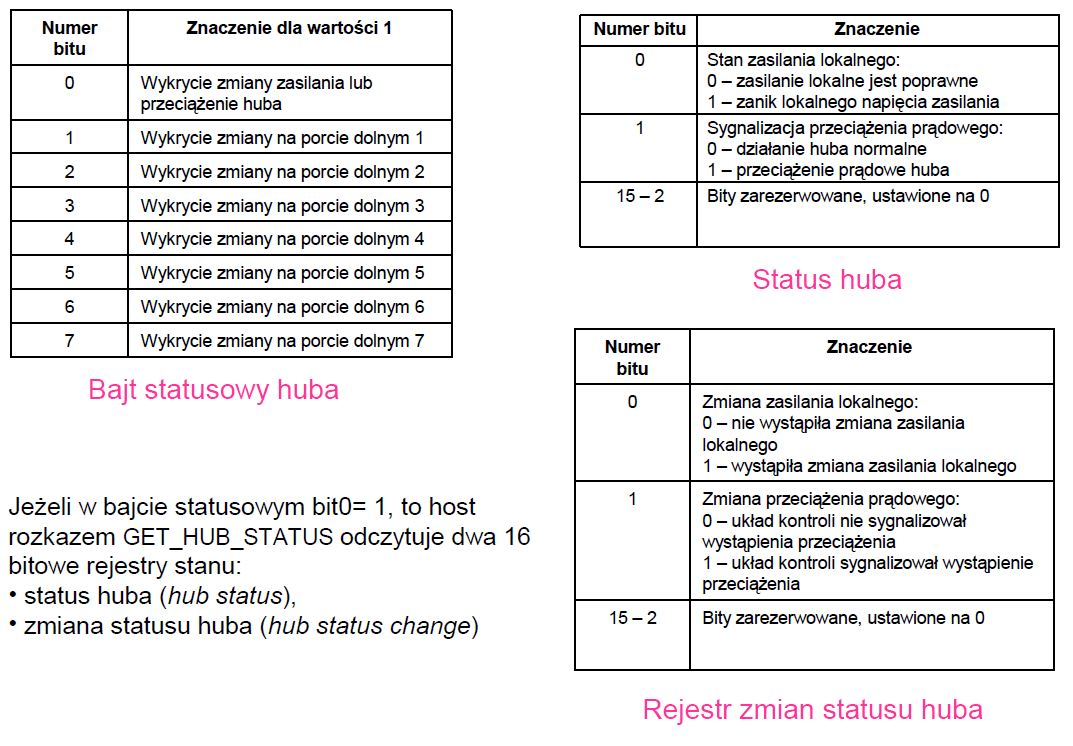
\includegraphics[width=8cm]{./wyklady/USB_35_1.jpg}
	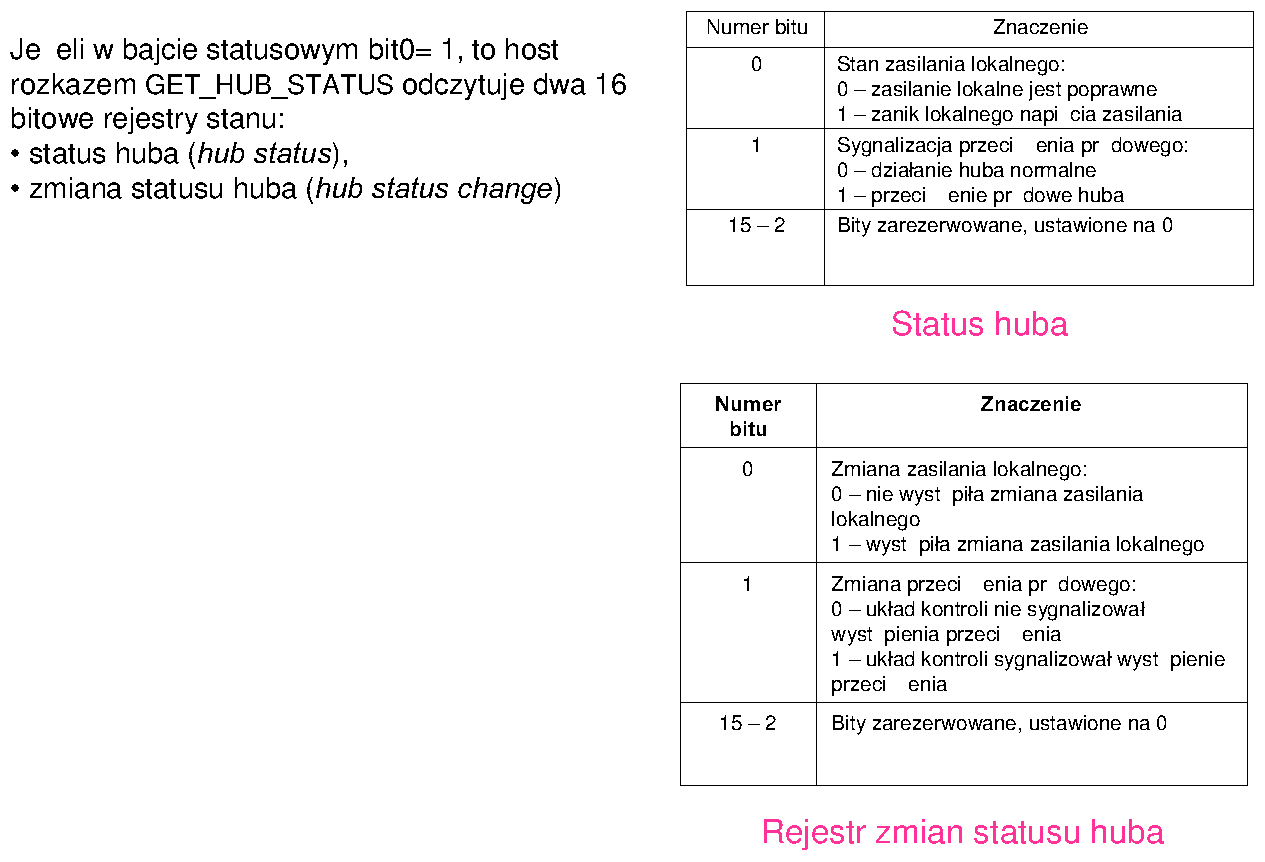
\includegraphics[width=8cm]{./wyklady/USB_36_1.jpg}
	
\subsection{Zasilanie urządzeń w systemie USB}
	USB jest również systemem dystrybucji i zarządzania zasilaniem urządzeń.
	\subsubsection{Możliwe zasilania urządzeń USB}
	\begin{itemize}
		\item Urządzenie zasilane z magistrali
		\item Urządzenie zasilane z własnego źródła
		\item Urządzenie zasilane częściowo z magistrali i własnego źródła
	\end{itemize}
	\subsubsection{Zasilanie hubów i pozostałych urządzeń}
		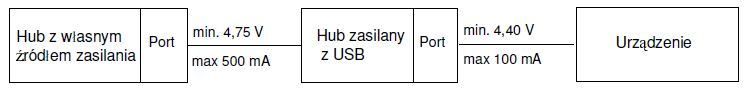
\includegraphics[width=11cm]{./wyklady/USB_38_1.jpg}\\
		Dopuszczalne spadki napięcia zasilania.
	\subsubsection{Urządzenie zasilane z magistrali}
		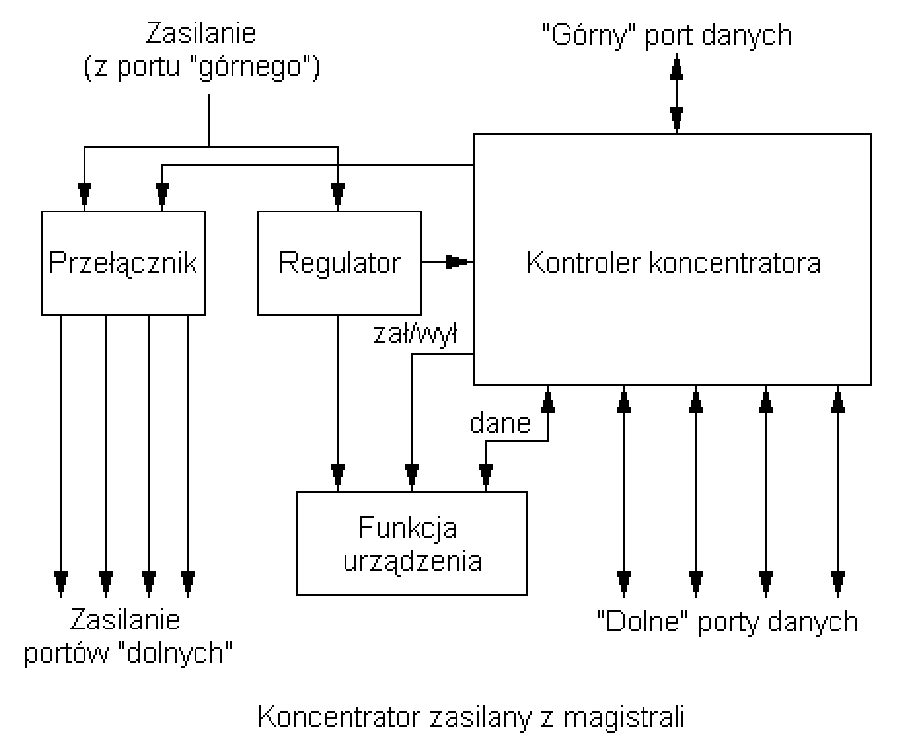
\includegraphics[width=7cm]{./wyklady/USB_39_1.pdf}\\
		Dla portu zasilanego z magistrali USB i podłączonego do portu o obciążalności 500 mA, 100 mA jest zarezerwowane na zasilanie jego układu. Oznacza to, że 400 mA pozostaje dla jego portów dolnych. Ponieważ każdy port musi mieć zapewnione minimum 100 mA, taki hub może mieć nie więcej niż 4 porty dolne (stąd pewnie przyjęty standard).
	\subsubsection{Zarządzanie zasilaniem}
	\begin{itemize}
		\item Wprowadzenie w \textbf{stan zawieszenia} pracy systemu – \emph{suspend}. Pozostając w zawieszenie urządzenie zachowuje swoją konfigurację, co pozwala jego wznowienie (\emph{resume}) do normalnego działania.
		\begin{itemize}
			\item \textbf{Globalne} (\emph{global suspend}) - rozkaz SetPortFeature (PORT\_SUSPEND) adresowany do huba głównego, zawiesza cały system
			\item \textbf{Częściowe} (\emph{selective suspend}) - rozkaz SetPortFeature (PORT\_SUSPEND) adresowany do huba zewnętrznego, w którym wybrany port (lub część systemu) ma zostać zawieszony. W ten sposób HUB zawiesza tylko siebie i poniższe HUBy/urządzenia.
			\item Zawieszone porty nie propagują ruchu „w dół” oraz nie przekazują „w górę” żadnych sygnałów od urządzeń do nich podłączonych.
			\item Urządzenia w stanie zawieszenia zachowują swój stan, co umożliwia wznowienie ich pracy bez ponownej konfiguracji.
			\item Hub w stanie zawieszenia dodatkowo blokuje wszystkie nadajniki, zatrzymuje wewnętrzne zegary i zachowuje stan wszystkich portów dolnych.
			\item Urządzenie w stanie zawieszenie pobiera prąd $< 500 [\mu A]$
			\item Urządzenie automatycznie przechodzi do stanu \emph{SUSPEND} po wykryciu braku aktywności magistrali przez 3 $ms$. (USB wysyła ramki co 1 ms)
			\begin{itemize}
				\item Urządzenia pełnej szybkości wykorzystują pakiety SOF
				\item Urządzenia małej szybkości wykorzystują generację przejścia ze stanu jałowego do stanu K w odstępach czasu nie większych niż 3 $ms$.
			\end{itemize}
		\end{itemize}
		\item \textbf{Wznowienie} pracy systemu - \emph{resume}
		\begin{itemize}
			\item Globalne
			\item Wake-up
			\item Wznowienie pracy urządzenia może nastąpić
			\newpage
			\begin{itemize}
				\item Z inicjatywy kontrolera - jako wznowienie po zawieszeniu globalnym lub częściowym\\
				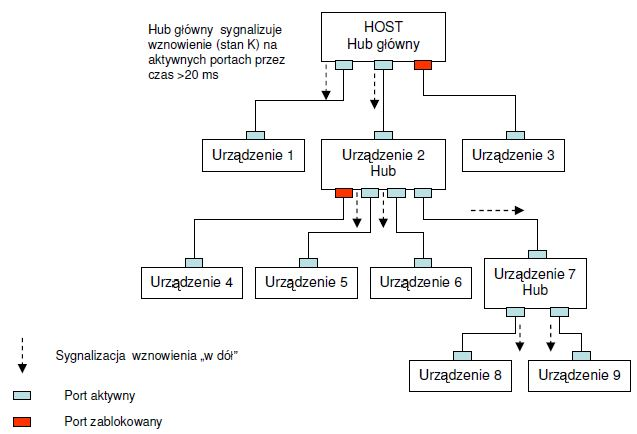
\includegraphics[width=7cm]{./wyklady/USB_43_1.jpg}
				\item Z inicjatywy urządzenia - po wystąpieniu zdarzenia wymagającego obsługi („budzenie” - \emph{Wakeup})\\
				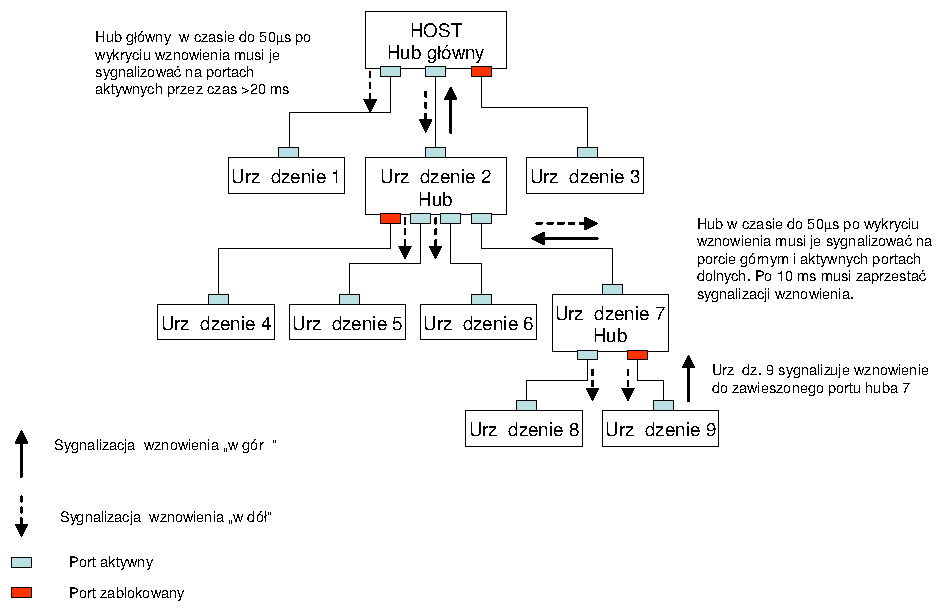
\includegraphics[width=7cm]{./wyklady/USB_44_1.jpg}
			\end{itemize}
			\item Wznowienie po zawieszeniu globalnym - rozpoczyna hub główny wykonując rozkaz wznowienia pracy systemu. Oznacza gotowość wszystkich hubów i urządzeń do wykonywania transakcji.
			\item Wznowienie po częściowym zawieszeniu - może wykonać:
			\begin{itemize}
				\item Host rozkazem \emph{ClearPortFeature} (PORT SUSPEND) adresowanym do huba w którym znajduje się zawieszony port.
				\item Urządzenie podłączone do zawieszonego portu poprzez \emph{Wakeup}
			\end{itemize}
		\end{itemize}
	\end{itemize}
	
\subsection{Rozwiązania host kontrolerów}
	\subsubsection{Co to jest?}
	Host kontrolera (\emph{Host Controller Driver}) przetwarza poszczególne IRP na transakcje, tworzy listę transakcji  w ramach ramki, przygotowuje scenariusz wykonania każdej transakcji i kontroluje jej wykonanie.
	\subsubsection{Rozwiązania}
	Opracowano dwa rozwiązania host kontrolera:
	\begin{itemize}
		\item Uniwersalny host kontroler - \emph{Universal Host Controler} (Intel)
		\item Otwarty host kontroler – \emph{Open Host Controler} (Compaq, Microsoft, National Semiconductor)
	\end{itemize}
	Są do siebie bardzo podobne, różnią się tylko sposobem obsługi oraz współpracą z hubem głównym.
	\subsubsection{Uniwersalny host kontroler (UHC)}
	\textbf{Zasada działania kontrolera UHC}\\
	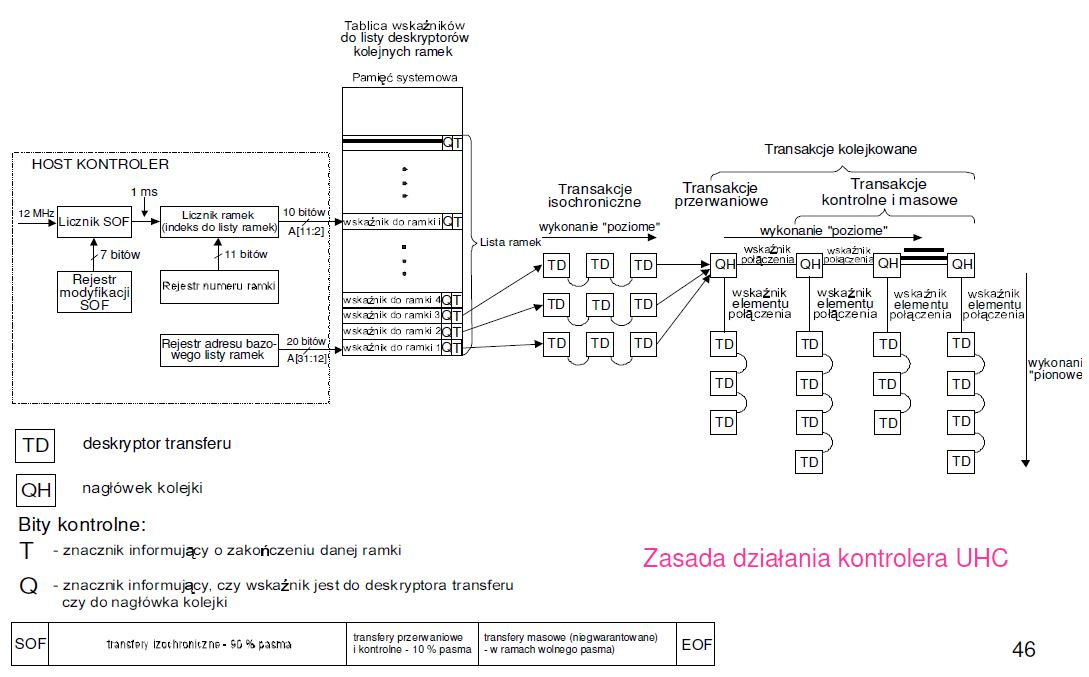
\includegraphics[width=12cm]{./wyklady/USB_46_1.jpg}\\\\
	\textbf{Ogólna postać deskryptora transferu (TD)}\\
	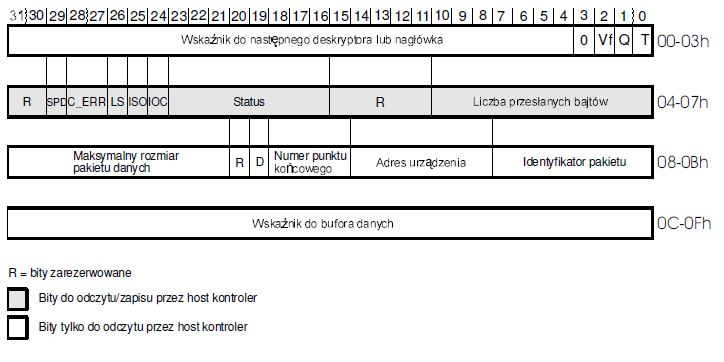
\includegraphics[width=12cm]{./wyklady/USB_47_1.jpg}\\\\
	\textbf{Ogólna postać nagłówka kolejki (QH)}\\
	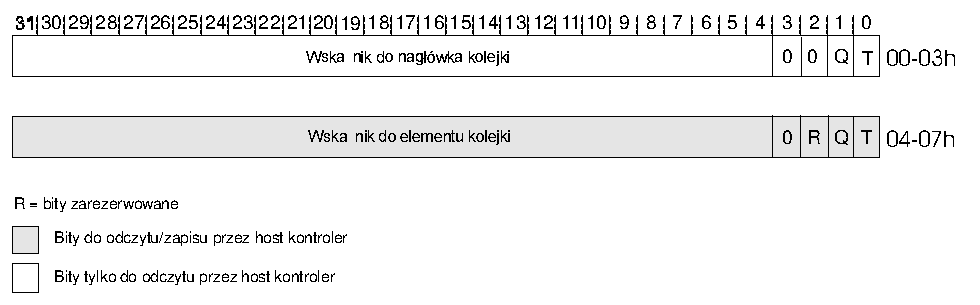
\includegraphics[width=12cm]{./wyklady/USB_48_1.pdf}
	\subsubsection{Otwarty host kontroler (OHC)}
	\textbf{Zasada działania kontrolera OHC}\\
	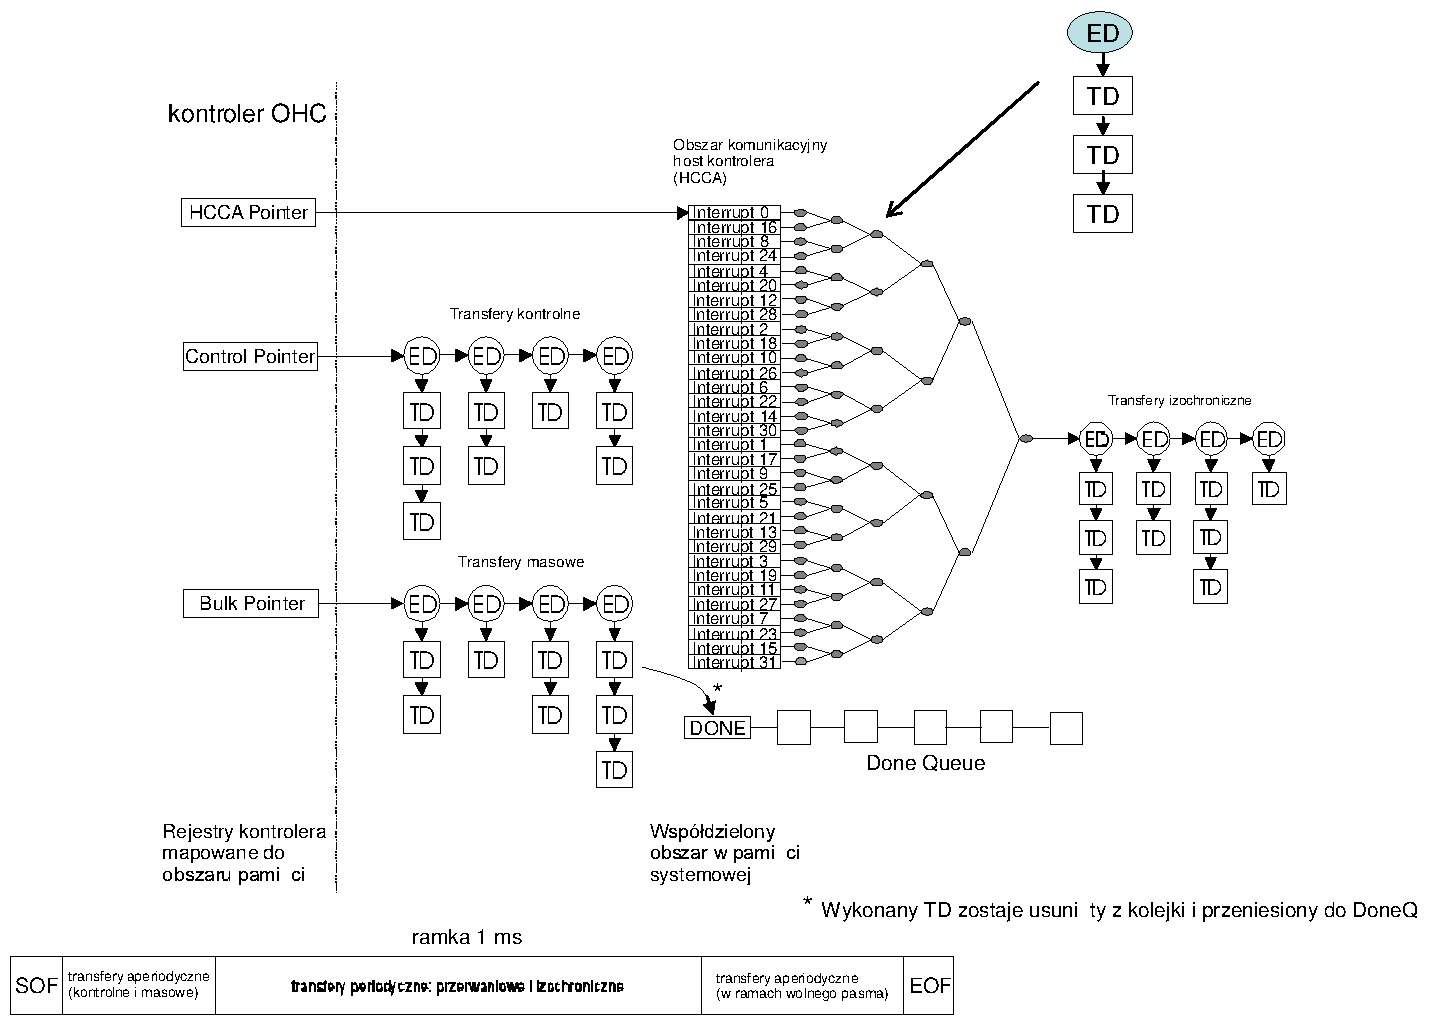
\includegraphics[width=12cm]{./wyklady/USB_49_1.pdf}\\\\
	\textbf{Format deskryptora punktu końcowego (ED)}\\
	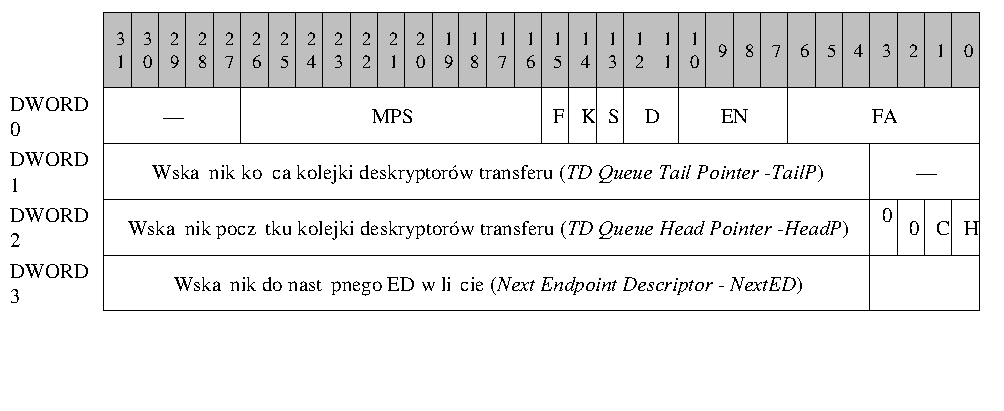
\includegraphics[width=12cm]{./wyklady/USB_50_1.jpg}\\\\
	\textbf{Ogólna postać deskryptora transferu (TD)}\\
	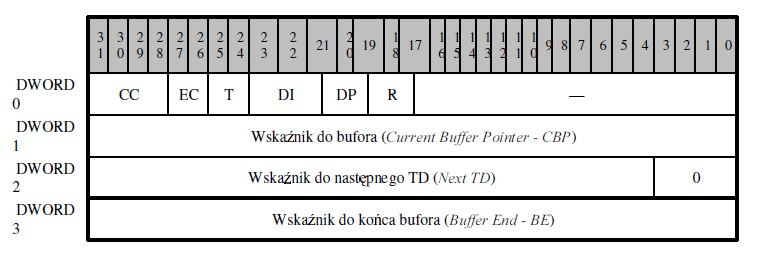
\includegraphics[width=12cm]{./wyklady/USB_51_1.jpg}
	\newpage
\subsection{USB 2.0 - rozszerzenie standardu}
	\subsubsection{Ważniejsze elementy wprowadzone w USB 2.0}
	\begin{itemize}
		\item Wysoka szybkość transmisji (high speed) - 480 Mb/s
		\item Protokół PING-NYET
		\item Transakcja SPLIT
		\item Komunikacja z szerokopasmowym punktem izochronicznym
		\item Nowe typy pakietów
	\end{itemize}
	\subsubsection{Wysoka szybkość transmisji}
	Podział ramki na 8 mikroramek wysokiej szybkości\\
	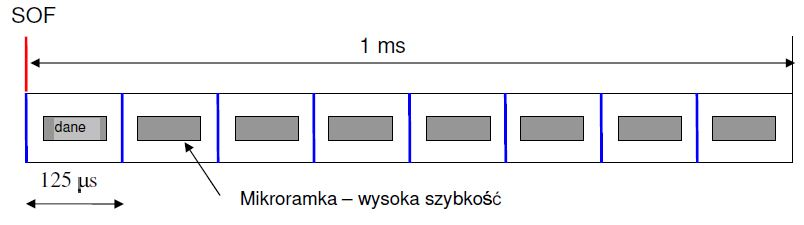
\includegraphics[width=7cm]{./wyklady/USB_53_1.jpg}
	\begin{itemize}
		\item Mikroramka trwa 125 $\mu s$
		\item Na 1 ramkę przypada 8 mikroramek
		\item Wysoka szybkość transmisji - w mikroramce wynosi 480 Mhz.
	\end{itemize}
	\subsubsection{Protokół PING-NYET}
	Potwierdzenie NYET (\emph{NOT YET}) dla urządzeń \emph{high speed}.\\
	\textbf{Problem:} przy zapisie do urządzenia, jeżeli nie jest ono „gotowe na dane” potwierdzenie negatywne przychodzi dopiero po pakiecie danych – strata czasu.\\
	\textbf{Rozwiązanie}:\\
	TOKEN PING – zapytanie urządzenia, czy jest gotowe do przyjścia danych.\\
	Możliwe odpowiedzi i reakcja hosta:
	\begin{itemize}
		\item ACK – wykonanie transakcji OUT
		\item NYET – host kontynuuje wysyłanie zapyta PING
	\end{itemize}
	\textbf{Korzyści}: lepsze wykorzystanie magistrali (PING jest krótki).
	\subsubsection{Transakcja SPLIT}
	\textbf{Problem:} Host i hub wysokiej szybkości komunikują się z urządzeniem małej lub pełnej szybkości. Szybkie przesyłanie danych pomiędzy hostem i hubem oraz wolne pomiędzy hubem i urządzeniem – konieczność buforowania danych w hubie.\\
	\textbf{Rozwiązanie}:\\
	Transakcja dzielona, złożona z dwóch części:
	\begin{itemize}
		\item SSPLIT (\emph{Start Split} - rozpoczęcie transakcji dzielonej)
		\item CSPLIT (\emph{Complete Split} – zakończenie transakcji dzielonej).
		\item Pomiędzy tymi dwoma elementami transakcji dzielonej mogą być wykonywane inne transakcje z wysoką szybkością.
	\end{itemize}
	\subsubsection{Komunikacja z szerokopasmowym punktem izochronicznym}
	Komunikacja z „normalnym” izochronicznym punktem końcowym zakłada jedną transakcję na ramę lub mikroramkę.\\
	W przypadku punktów szerokopasmowych, obsługiwanych tylko przez kanały \emph{high speed}, istnieje możliwość przekazania w jednej mikroramce większej ilości danych wykonując bezpośrednio po sobie od jednej do trzech transakcji.\\
	Dane w takiej sekwencji transakcji muszą być oznaczone, przy czym nie wystarczą już „znaczniki” Data 0 i Data 1, dlatego wprowadzono dwa kolejne typy pakietów danych: \textbf{Data 2} i \textbf{MData}.\\
	Pakiet \textbf{Data 2} wykorzystywany jest przy odczycie danych z urządzenia, natomiast \textbf{MData} i \textbf{Data 2} przy zapisie do urządzenia.\\
	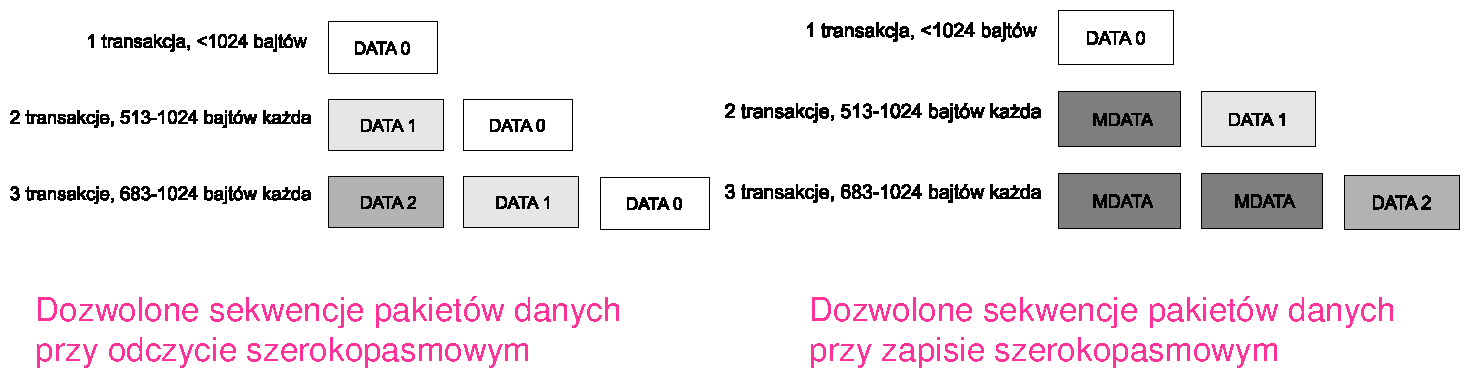
\includegraphics[width=15cm]{./wyklady/USB_56_1.pdf}
	\subsubsection{Specjalne pakiety TOKEN wprowadzone w USB 2.0}
	Kody pakietów specjalnych zgodnie z USB 2.0\\
	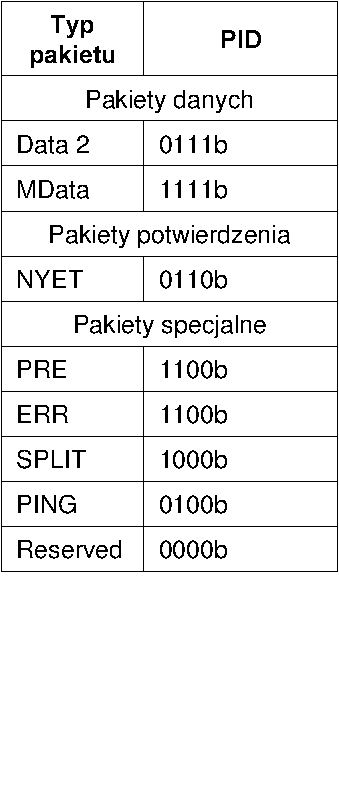
\includegraphics[width=3cm]{./wyklady/USB_57_1.pdf}